\begin{frame}
\frametitle{Blockclustering: Clustering \& Admissibility}
It is a quad-tree whose nodes are matrix blocks and the leaves are admissible (or small) blocks; a block is split in a $2 \times 2$ block structure. 
\begin{table}[ht]
\centering
\begin{tabular}{cc}
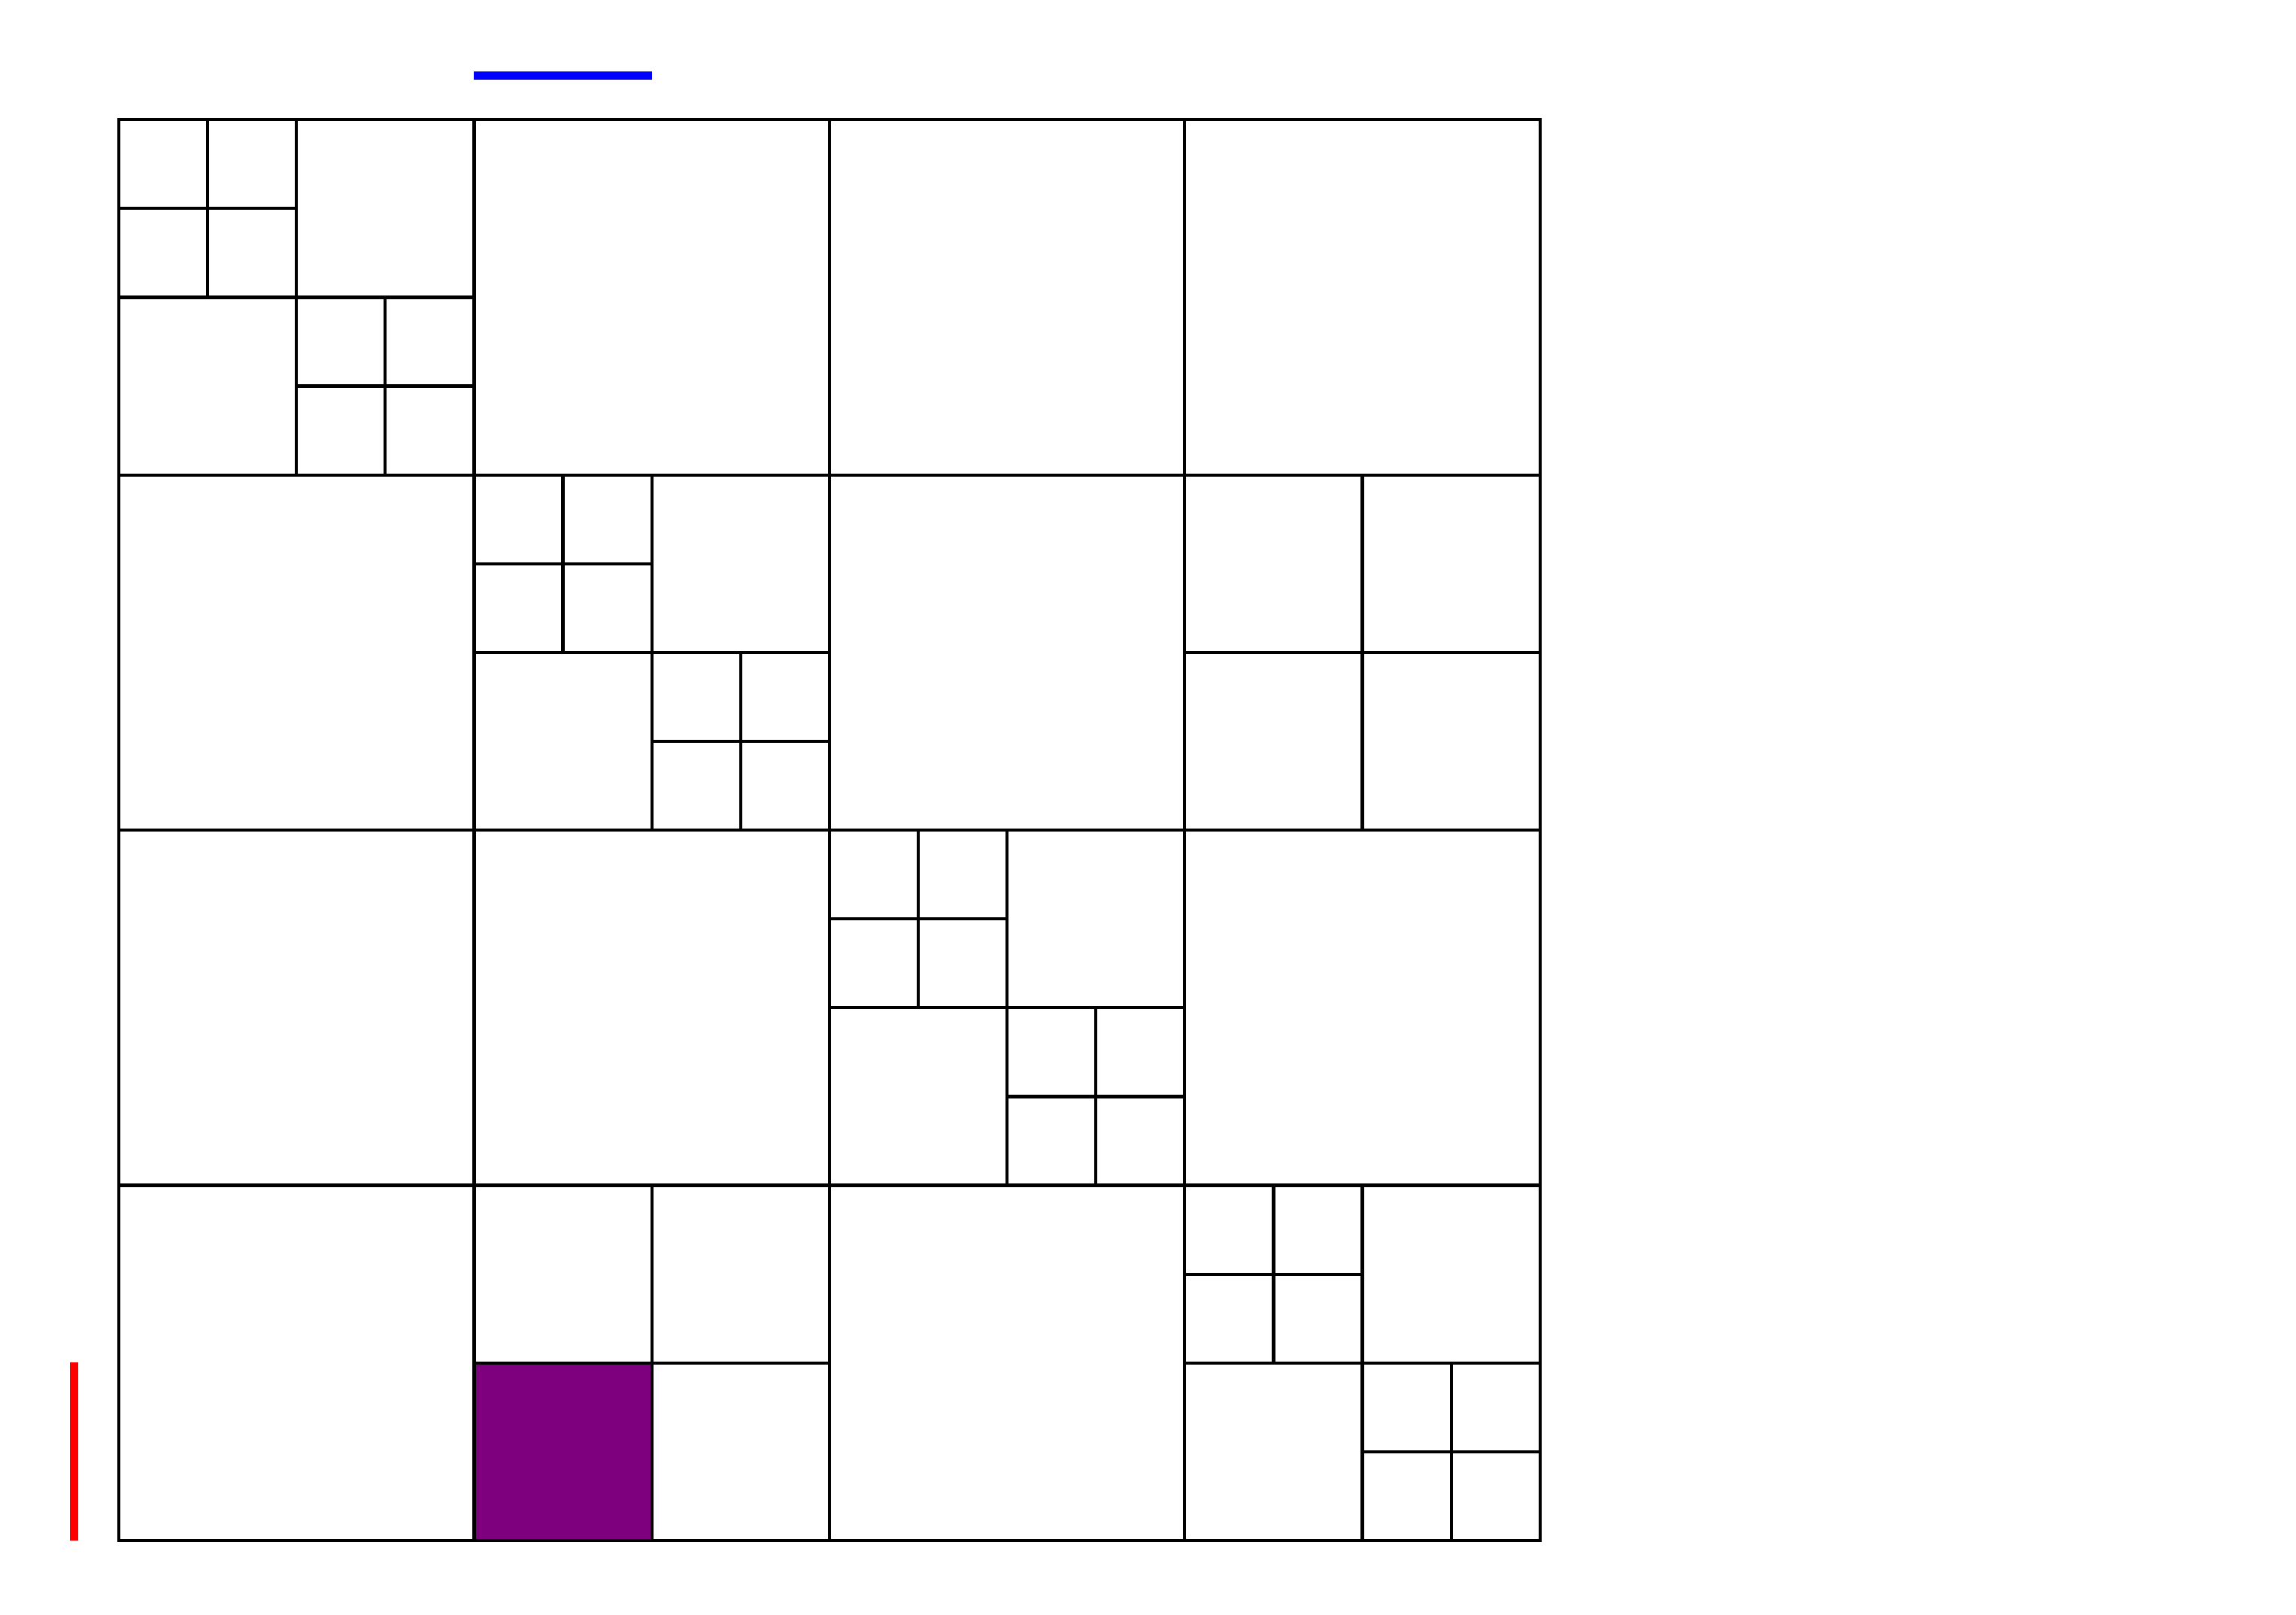
\includegraphics[scale=0.4]{./img/BlockClusteringA.png} & 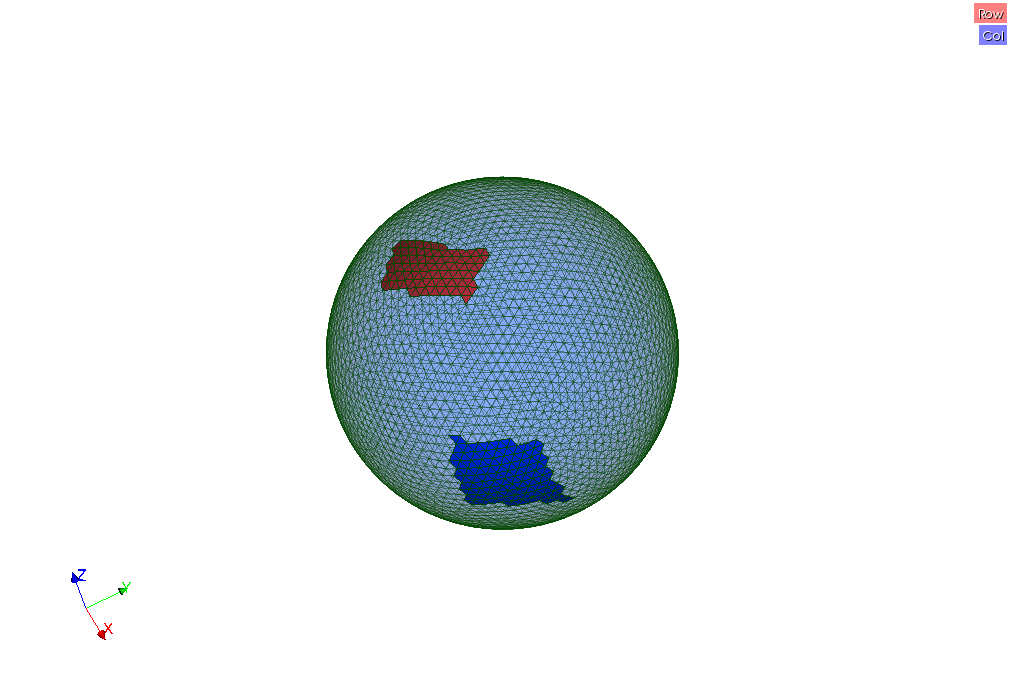
\includegraphics[scale=0.244]{./img/BlockClusteringB.png}
\end{tabular}
\caption{Blockclustering and the geometry}
\end{table}
\end{frame}

\begin{frame}
\frametitle{The \hmat structure}

A \hmat  is a \textbf{quadtree} (with Binary Space Partitioning):
\begin{itemize}
\item Internal nodes: subdivided \hmat; 
\item Leaves:
\begin{itemize}
\item admissible block: large \& low-rank;
\item inadmissible block: dense \& full rank, but small.
\end{itemize}

\begin{block}{Remarks}
\begin{itemize}
\item Only the leaves carry data; 
\item Big admissible blocks ($10^4 \times 10^4$ and more)
\item Small (and few) inadmissible blocks ($100 \times 100$).
\end{itemize}
\end{block}

\end{itemize}

Each admissible block is compressed with a fast method thus determining a numerical rank with  a prescribed relative error {$\varepsilon$}.

\end{frame}

